\documentclass[12pt]{article}

\usepackage[a4paper,margin=0.5in]{geometry}

\usepackage[square,numbers,sort&compress]{natbib}
%\usepackage[sort&compress]{natbib}

\usepackage[utf8]{inputenc} % allow utf-8 input
\usepackage[T1]{fontenc}    % use 8-bit T1 fonts
\usepackage{hyperref}       % hyperlinks
\usepackage{url}            % simple URL typesetting
\usepackage{booktabs}       % professional-quality tables
\usepackage{amsfonts}       % blackboard math symbols
\usepackage{nicefrac}       % compact symbols for 1/2, etc.
\usepackage{microtype}      % microtypography
\usepackage{amsmath}
\usepackage{algorithm}
\usepackage[noend]{algpseudocode}

\usepackage{times}
\usepackage{amsfonts}
\usepackage{amsmath}
\usepackage[psamsfonts]{amssymb}
\usepackage{latexsym}
\usepackage{color}
\usepackage{graphics}
\usepackage{enumerate}
\usepackage{amstext}
\usepackage{blkarray}
\usepackage{url}
\usepackage{epsfig}
\usepackage{bm}
\usepackage{hyperref}
\hypersetup{
    colorlinks=true,
    linkcolor=blue,
    filecolor=magenta,      
    urlcolor=blue,
}
\usepackage{mathtools}

\usepackage{graphicx}
\newcommand{\bigo}[1]{{\cal O}\left(#1 \right)}
\newcommand{\p}[1]{\mathrm{P}\left(#1 \right)}
\newcommand{\tr}{^\mathrm{t}}

\newcommand{\matr}[1]{\bm{#1}}     % ISO complying version
\newcommand{\vect}[1]{\mathbf{#1}}

\begin{document}
\thispagestyle{empty}
\begin{center}

\textbf{DS-GA 3001.001 Special Topics in Data Science: Modeling Time Series\\
Homework 2}
\end{center}

\noindent Yves Greatti - yg390\\

\noindent \textbf{Problem 1.} LDS model, 10p \\ %10
Consider a special case of LDS with $\vect{C} = \vect{I}$ and  $\vect{R} = \sigma^2 \vect{I}$, where $\vect{I}$ denotes the identity matrix. 
Show that in the limit where there is no observation noise the best estimate for latent $\vect{z}_i$ is to simply use the observation $\vect{x}_i$: 
formally, in the limit when $\sigma^2 \rightarrow 0$ the posterior for $\vect{z}_i$ has mean $\vect{x}_i$ and vanishing variance.\\
Given the LDS model specifications for the posterior $\vect{z}_i$:
\begin{align*}
	\mu_{i|i}		&= 	\mu_{i|i-1} + \matr{K}_i (\vect{x}_i - \matr{C} \mu_{i|i-1}) \\
	\Sigma_{i|i}	&=	\Sigma_{i|i-1} - \matr{K}_i 	 \matr{C}  \Sigma_{i|i-1}
\end{align*}
where $ \matr{K}_i = \Sigma_{i|i-1}	 \matr{C} ^T ( \matr{C} \Sigma_{i|i-1}  \matr{C} ^T + \matr{R})^{-1}$. If $\vect{C} = \vect{I}$ and  $\vect{R} = \sigma^2 \vect{I}$, then the Kalman gain becomes
 $ \matr{K}_i = \frac{\Sigma_{i|i-1}} {\Sigma_{i|i-1} + \sigma^2 \vect{I}} $, taking the limit  $\sigma^2 \rightarrow 0$ then $ \matr{K}_i \rightarrow \vect{I}$, thus in the limit the posterior $\vect{z}_i$ has for parameters:
\begin{align*}
	\mu_{i|i}		&= 	\mu_{i|i-1} + (\vect{x}_i - \mu_{i|i-1})  = \vect{x}_i \\
	\Sigma_{i|i}	&=	\Sigma_{i|i-1} -  \Sigma_{i|i-1} = \vect{0}
\end{align*}


\noindent \textbf{Problem 2. } LDS prediction, 10p \\%20
Given the standard parametrization of the LDS model, and the Kalman filtering estimates $\mu_{i|i}$ and $\Sigma_{i|i}$, obtained for a dataset $\vect{x}_{1:t}$ write down the expressions 
for predicting the following 2 observations in the sequence $\vect{x}_{t+1}$ and  $\vect{x}_{t+2}$.\\
Given the prior with parameters  $\mu_{i|i}$ and $\Sigma_{i|i}$, we compute the prior for $\vect{z}_{t + 1} \approx \mathcal{N} (\mu_{i+1|i}, \Sigma_{i+1|i})$:
\begin{align*}
	\mu_{i+1|i}	&= 	\matr{A} \mu_{i|i} \\
	\Sigma_{i+1|i}	&=	 \matr{A}  \Sigma_{i|i}  \matr{A}^t + \matr{Q}
\end{align*}
We obtain the prediction $\vect{x}_{t+1} \approx \mathcal{N} (\matr{C} \mu_{i+1|i}, \matr{C} \Sigma_{i+1|i} \matr{C}^t + \matr{R} )$, we then incorporate the evidence to obtain the posterior parameters:
\begin{align*}
	\mu_{i+1|i+1}		&= 	\mu_{i+1|i} + \matr{K}_{i+1} (\vect{x}_{t+1} - \matr{C} \mu_{i+1|i}) \\
	\Sigma_{i+1|i+1}	&=	\Sigma_{i+1|i} - \matr{K}_{i+1} 	 \matr{C}  \Sigma_{i+1|i}
\end{align*}
where the Kalman gain matrix $ \matr{K}_{i+1} = \Sigma_{i+1|i}	 \matr{C} ^t ( \matr{C} \Sigma_{i+1|i}  \matr{C} ^t + \matr{R})^{-1}$
which we use to update the posterior $\vect{z}_{t+1} \approx \mathcal{N} (\mu_{i+1|i+1},\Sigma_{i+1|i+1})$.
With the updated  $\vect{z}_{t+1}$ we can compute the next prior $\vect{z}_{t + 2} \approx \mathcal{N} (\mu_{i+2|i+1}, \Sigma_{i+2|i+1})$ where 
\begin{align*}
	\mu_{i+2|i+1}		&= 	\matr{A} \mu_{i+1|i+1} \\
	\Sigma_{i+2|i+1}	&=	 \matr{A}  \Sigma_{i+1|i+1}  \matr{A}^t + \matr{Q}
\end{align*}
which is used to obtain the prediction  $\vect{x}_{t+2} \approx \mathcal{N} (\matr{C} \mu_{i+2|i+1}, \matr{C} \Sigma_{i+2|i+1} \matr{C}^t + \matr{R} )$.
 
\noindent \textbf{Problem 3.} LDS inference with missing observations, 10p \\%20
Consider a variation of the original LDS graphical model with one single missing value $\mathbf{x}_j$. Everything else is as in the original; the only difference is that the graphical model loses the downward observation arrow and the corresponding $\mathbf{x}_j$.)
How do the Kalman filtering/smoothing updates change?\\

When the observation $\vect{x}_j$ is missing the update  $\vect{x}_j$ and the Kalman gain $\matr{K}_i$ are zero. Filtering equations become:
\begin{align*}
			\mu_{j|j}		&= \mu_{j | j-1 }		= \matr{A}  \mu_{j-1| j-1} \\
			\Sigma_{j|j}	&= \Sigma_{j|j-1}	=  \matr{A}  \Sigma_{j-1|j-1}  \matr{A}^t  +  \matr{Q} 
 \end{align*}
And the smoothing equations are now:
\begin{align*}
			\mu_{j|t}		&=	\matr{A}  \mu_{j-1| j-1} + \matr{F}_j (\mu_{j+1|t}  - \mu_{j+1|j}) = \matr{A} \mu_{j-1|j-1}  + \matr{F}_j (\mu_{j+1|t} - \matr{A} \mu_{j|j}) \\
			\Sigma_{j|t}	&=	 \Sigma_{j|j}	+ \matr{F}_j (\Sigma_{j+1|t}  - \Sigma_{j+1|j})   \matr{F}_j^t \\
			 \matr{F}_j		&= 	\Sigma_{j|j}	 \matr{A}^t  \Sigma_{j+1|j}^{-1}	= (\matr{A}  \Sigma_{j-1|j-1}  \matr{A}^t  +  \matr{Q} )	 \matr{A}^t   
			 				(\matr{A}  \Sigma_{j|j}  \matr{A}^t  +  \matr{Q} )^{-1}	
 \end{align*}
We can recursively express $\mu_{j+1|j}$ , $\Sigma_{j|j}$ in term of $\Sigma_{j-1|j-1}$ in both $\mu_{j|t}$ and $\Sigma_{j|t}$  up to $\mu_0$ and $\Sigma_0$. 
So $\mu_{j|t}$ and  $\Sigma_{j|t}$ are reduced with the exceptions of the terms $\mu_{j+1|t}$ and $\Sigma_{j+1|t}$,  
to matrix multiplications of $\matr{A}$ , $ \matr{Q}$, $\mu_0$ and $\Sigma_0$. 
\\

\noindent \textbf{Problem 4.}  LDS filtering, 10p\\ 
Given the model parameters: $A = 
\begin{bmatrix} %0.9 0.1; 0.3 0.7
0.65 &   0.3\\
    0.2   & 0.8
\end{bmatrix}
$,
$C= 
\begin{bmatrix}  
    1.1 & 0.2\\
    0.5 & 0.95\\
\end{bmatrix},\\
$
$Q= 0.1 \vect{I}_2$, 
$R= 0.01 \vect{I}_2$ with initial condition parameters $\mu_0 = [0\; 0]^\mathrm{t}$, $\Sigma_0 = 0.5 \vect{I}$.
Generate 25 samples from the model and  plot them. Use these observation for inference (filtering and smoothing). How much does the Kalman gain $\mathbf{K}_i$, and $\mathbf{F}_i$ vary across timepoints? Try playing around with the parameters. Does the result change? Discuss.\\
Note: you can use code from the lab as starting point, if you want. Not need to submit the code, only your figures.
\\

With the given parameters, using the code from the lab, the sampling of 25 observations gives us the plots below:
\begin{center}
	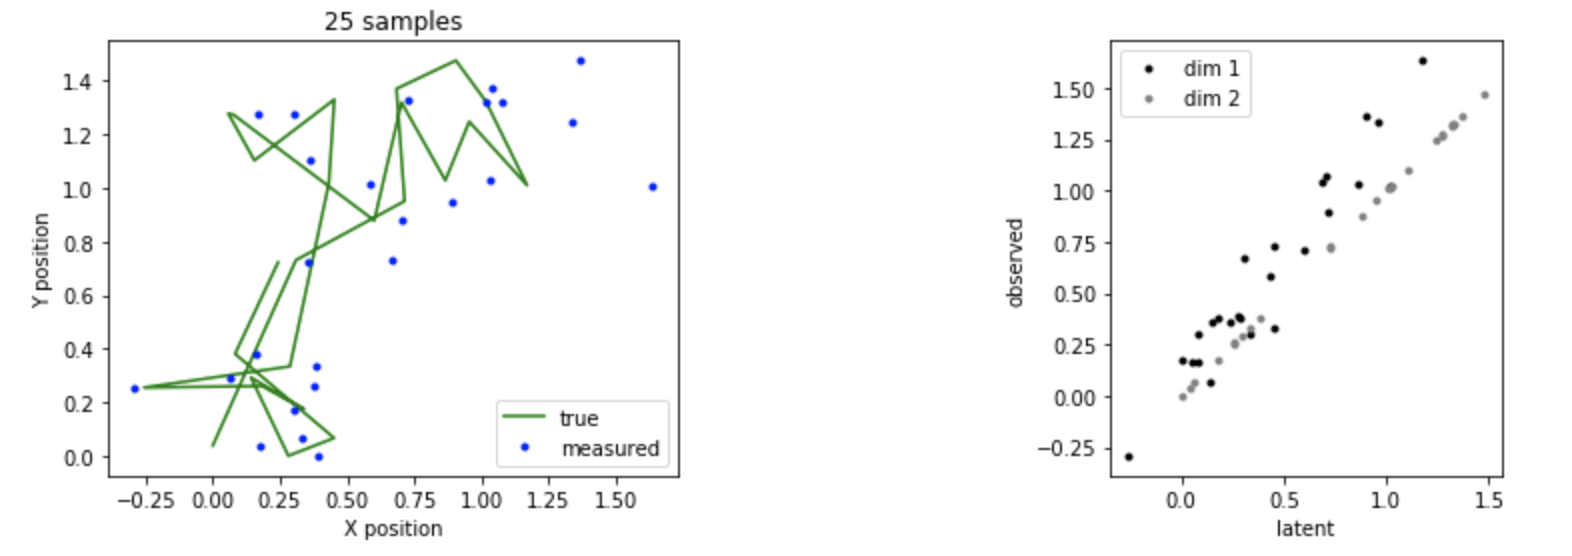
\includegraphics[width=1\linewidth]{figures/problem_4_1.png} 
\end{center}

After inference (filtering and smoothing) we obtain the estimates in red:
\begin{center}
	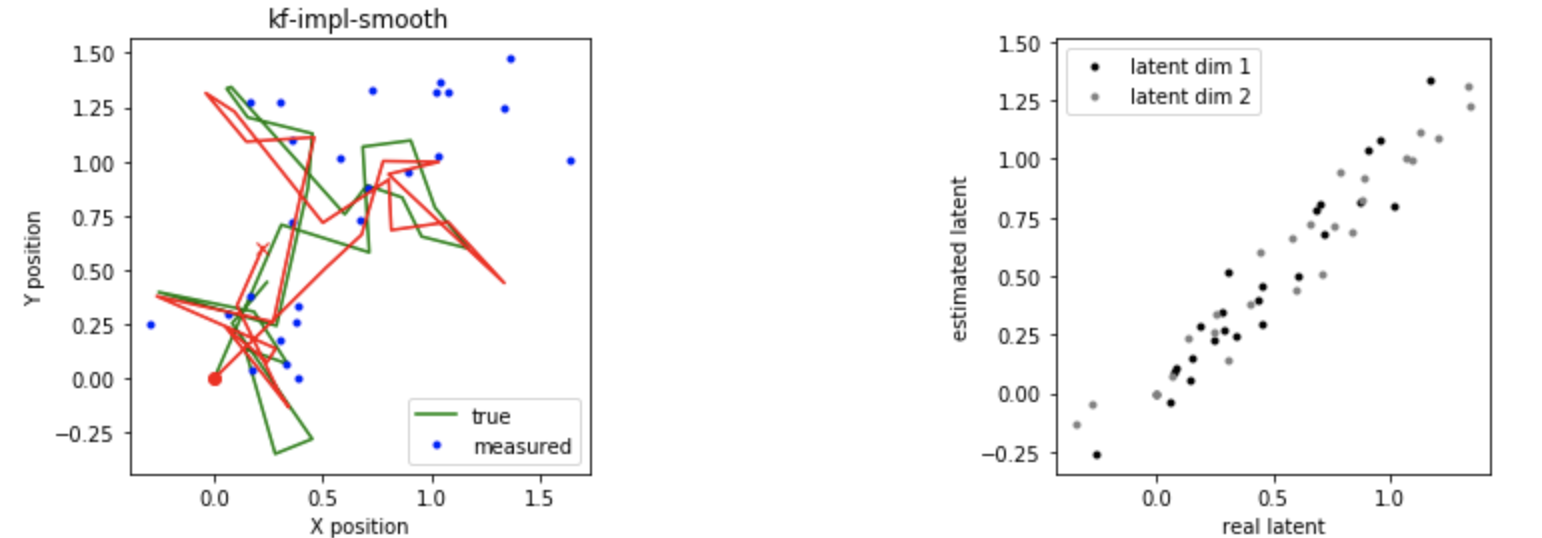
\includegraphics[width=1\linewidth]{figures/problem_4_2.png} 
\end{center}

At iteration $i$, Kalman gain is the matrix $\mathbf{K}_i = \Sigma_{i|i-1} \matr{C}^t (\matr{C} \Sigma_{i|i-1}\matr{C}^t  + \matr{R})^{-1}$ and the "smooth" gain $\mathbf{F}_i = 
\Sigma_{i|i} \matr{A}^t \Sigma_{i+1|i}^{-1}$.
At each time step, we compute the frobenius norm: $|\|A\|_{\mathrm{F}}=\sqrt{\sum_{i=1}^{m} \sum_{j=1}^{n}\left|a_{i j}\right|^{2}}=\sqrt{\operatorname{trace}\left(A^{*} A\right)}=\sqrt{\sum_{i=1}^{\min \{m, n\}} \sigma_{i}^{2}(A)}$ 
of the Kalman gain and F matrices and we plot them. On the plots below, we can see that once established since the system is linear, the Kalman matrix does not change.
\begin{center}
	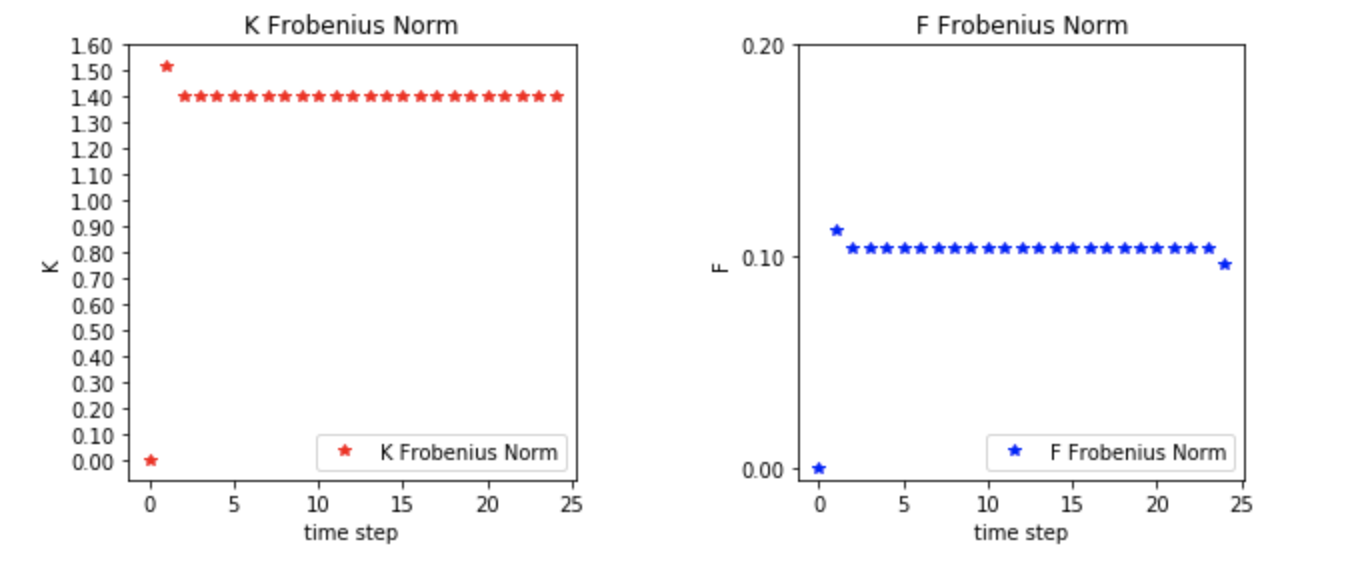
\includegraphics[width=1\linewidth]{figures/problem_4_3.png} 
\end{center}

The intuition behind the Kalman gain are:
\begin{enumerate}
	\item The more noisy the measurement is, the less precise it is. Hence, the innovation that represents the bias in the measurement may not be real innovation but rather an artifact of the measurement noise. Noise or uncertainty is directly captured by variance. Thus the larger the measurement variance noise, the lower the Kalman gain should be.
	\item The more noisy the process state is, the more important the innovation should be taken into account. Hence, the larger the process state variance, the larger the Kalman gain should be.
Summarizing these two intuitions, we would expect the Kalman gain to be:
\[
	\matr{K}_i = \frac{ \text{Process Noise}}{ \text{Measurement Noise}}
\]
\end{enumerate}
Using a smoother dynamic system, we confirm the intuition experimentally, as described below, we vary different parameters and observe the results listed below:
\begin{center}
	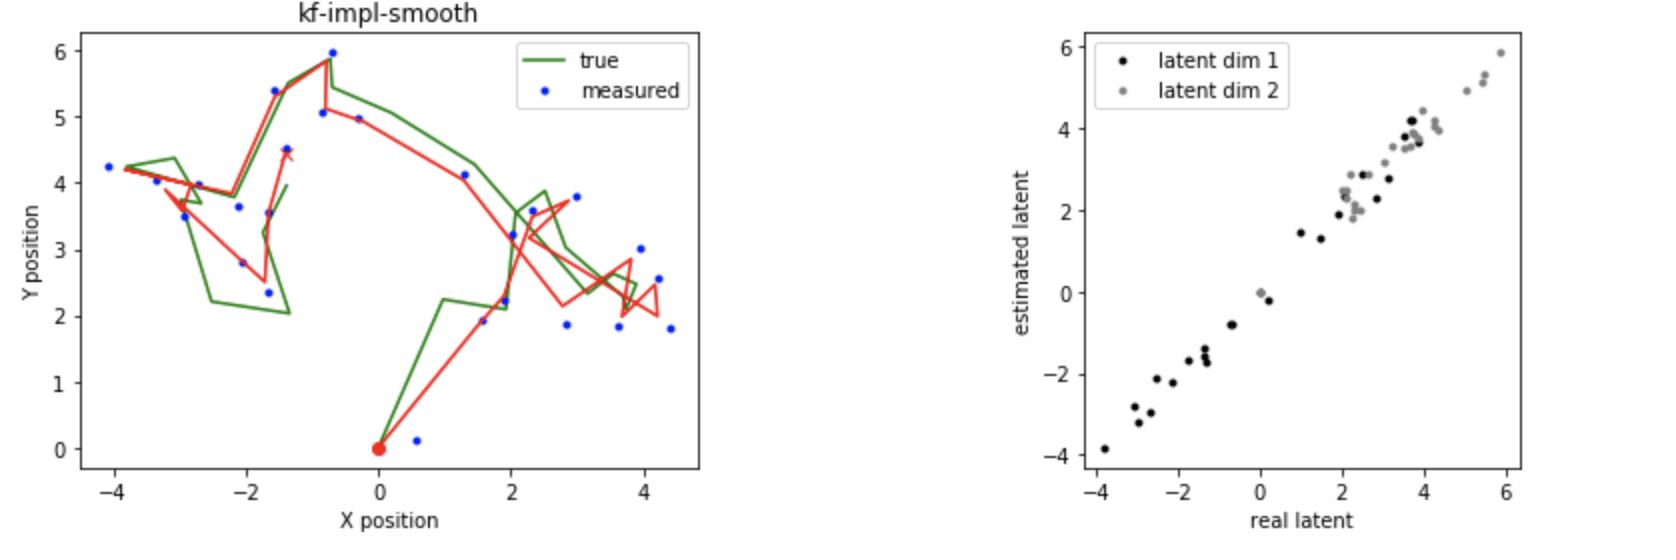
\includegraphics[width=1\linewidth]{figures/problem_4_4.png} 
\end{center}
\begin{center}
	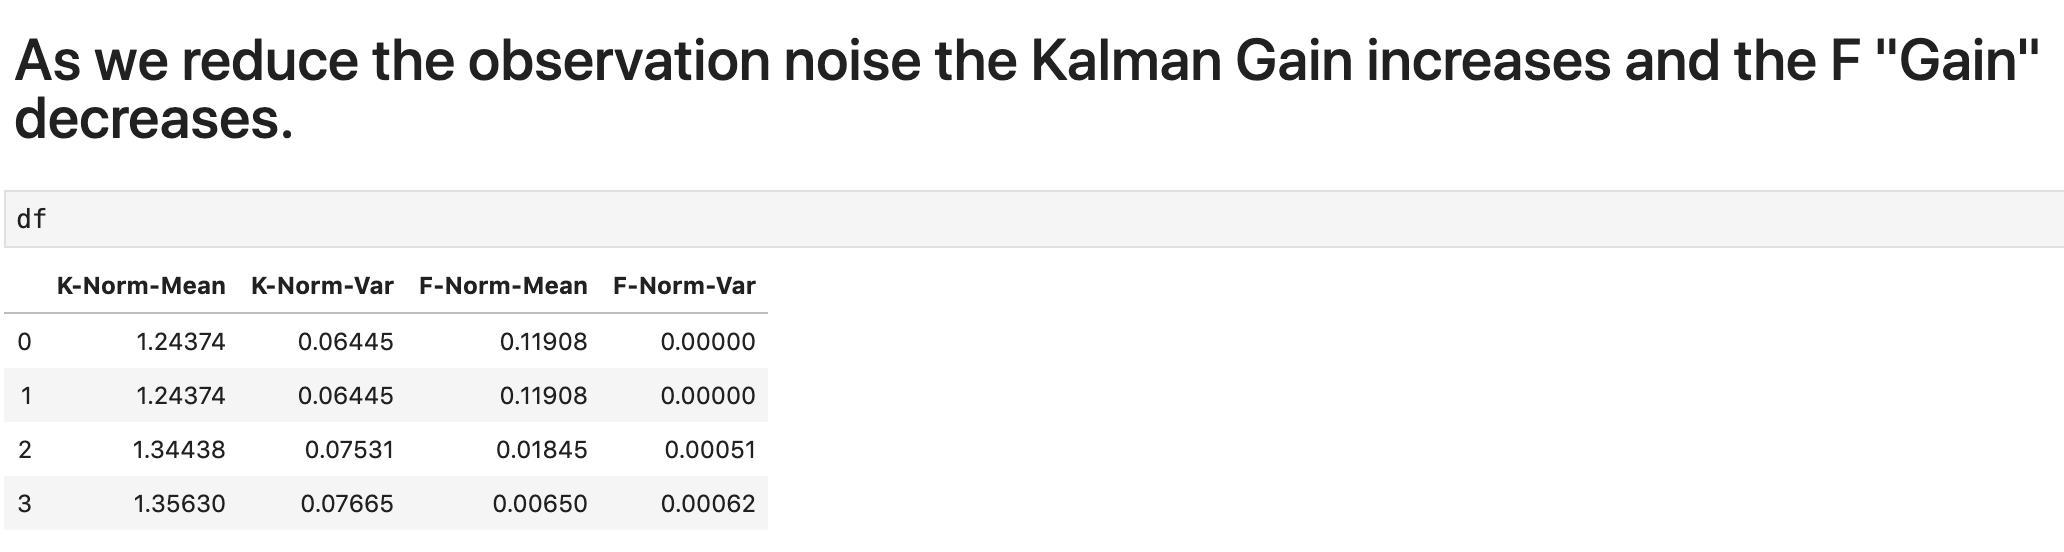
\includegraphics[width=1\linewidth]{figures/problem_4_5.png} 
\end{center}
\begin{center}
	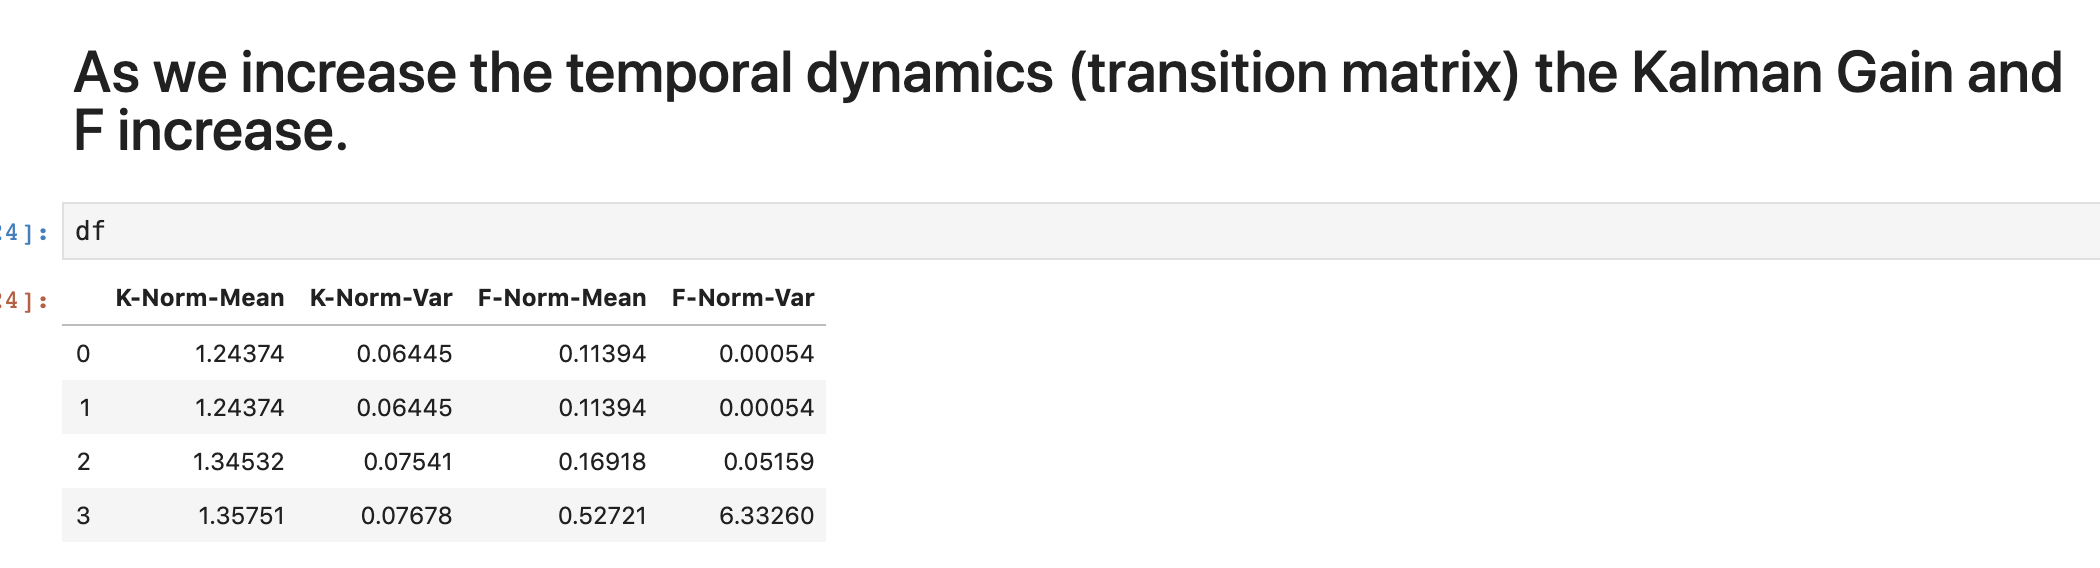
\includegraphics[width=1\linewidth]{figures/problem_4_6.png} 
\end{center}
\begin{center}
	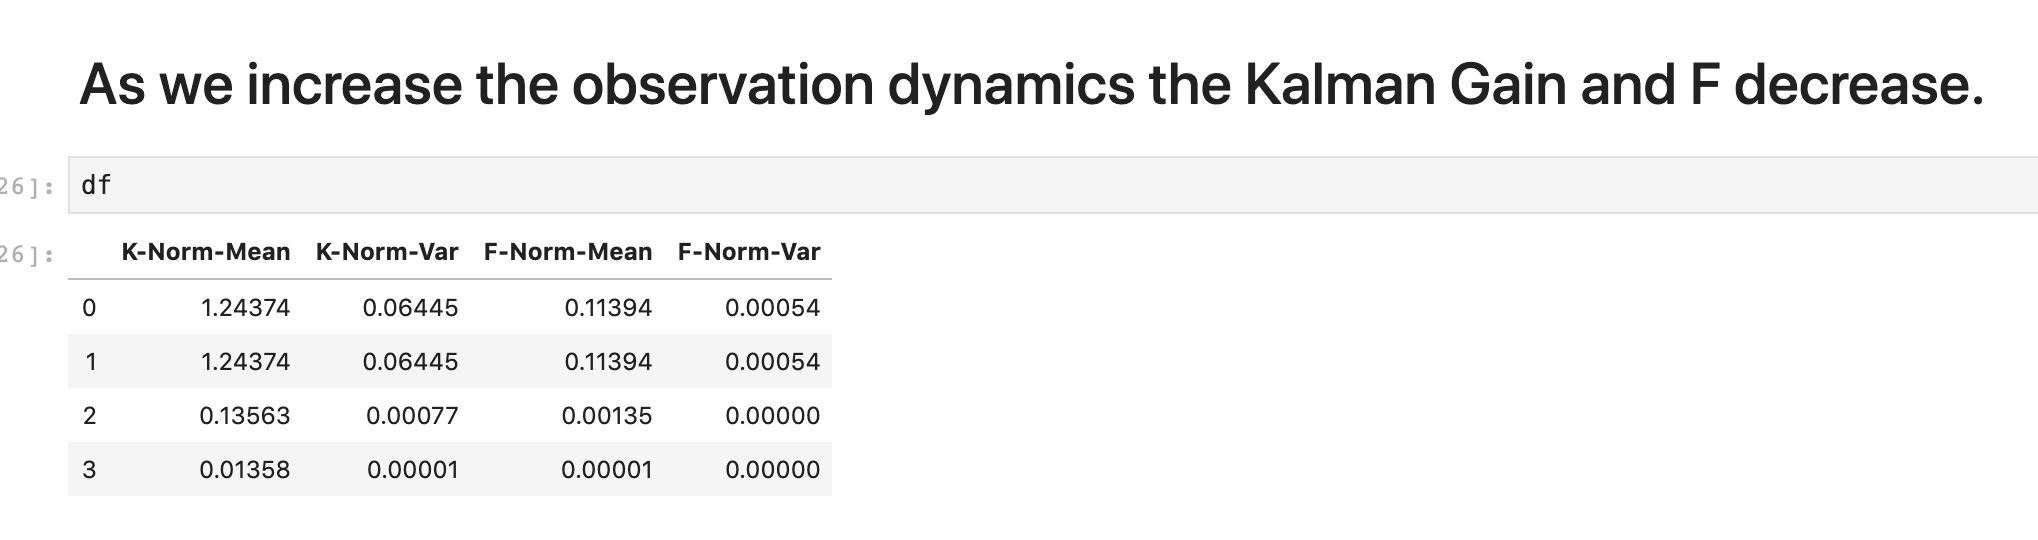
\includegraphics[width=1\linewidth]{figures/problem_4_7.png} 
\end{center}

\noindent \textbf{Problem 5 }  Particle filtering, 10p\\%20
Consider the usual LDS model, but where inference is done using particle filtering instead of the traditional Kalman filter. Write down pseudocode for the particle updates. Given the generated samples, $\{\mathbf{z}_i^{(k)}\}_{k=1:K, i=1:t}$, how would you go about computing the quantities $\mu_{i|i}$, $\Sigma_{i|i}$ and $\mathbb{E}[\mathbf{z}_i \mathbf{z}_{i+1}^t]$?\\
Hint: Use the general form from the lecture, and plug in the expressions for the different probabilities of the LDS model. The mean and variance can be written as expectations and approximated accordingly.
\end{document}